\chapter{Introducción}


${ }$\\
\section{Rigidez, ovaloides y otros conceptos y resultados previos}
${ }$\\
${ }$\\


Para llegar al resultado principal que se pretende demostrar primero vamos a ver algunos resultados y definiciones que son necesarios para comprender un poco mejor lo que se quiere mostrar. Algunos de estos resultados no estarán demostrados debido a que se alejan del propósito de este trabajo.
${ }$\\



${ }$\\
\subsection{Preliminares}
${ }$\\


La definición de superficie que aquí se va a tratar es la de aquella que es un subconjunto de $\mathbb{R}^3$ tal que para cada uno de sus puntos existe un entorno que lo contiene y es similar a una pieza de plano que se dobla suavemente y sin intersecciones cuando es doblado en $\mathbb{R}^3$. La definición formal es la siguiente:
${ }$\\

\begin{definicion}
	Diremos que $S \subset \mathbb{R}^3$ es una \underline{\textbf{superficie}} si para todo $p \in S$ existe un entorno $V \subset S$ de $p$, un abierto $U \subset \mathbb{R}^2$ y una aplicación $X : U \to \mathbb{R}^3$ diferenciable tales que:
	\begin{enumerate}
		\item $X(U) = V$,
		\item la aplicación $X : U \to V$ es un homeomorfismo,
		\item $\forall x \in U$, $(dX)_x : \mathbb{R}^2 \to \mathbb{R}^3$ es inyectiva.
	\end{enumerate}
\end{definicion}
${ }$\\

Al plano vectorial $(dX)_x(\mathbb{R}^2)$ le llamaremos el plano tangente a $S$ en el punto $q = X(x)$. Lo representaremos por $T_q S$.
${ }$\\

Los movimientos rígidos cumplen $\langle f(u), f(v) \rangle = \langle u, v \rangle$, siendo $<,>$ la métrica Euclídea de $\mathbb{R}^3$. Por lo que más intuitivamente podemos decir que, la distancia entre puntos (siendo la distancia la longitud de la linea recta que los une), se conserva al aplicar $f$.
${ }$\\

\begin{definicion}
	Llamaremos \underline{\textbf{movimiento rígido}} de $\mathbb{R}^3$ a una aplicación $f : \mathbb{R}^3 \to \mathbb{R}^3$ de la forma $f(x) = Ax + b$ donde A es una matriz ortogonal de orden 3 y $b \in \mathbb{R}^3$, es decir $A \in O(3)$ con lo cual cumple que $AA^{t} = I_{n}$.
\end{definicion}
${ }$\\


\begin{definicion}\label{def:isom} % label para cuando haga una referencia.
	Dadas dos superficies S y $S'$ y dada una aplicación $f : S \longrightarrow S'$, diremos que $f$ es una \underline{\textbf{isometría}} si es un difeomorfismo y además conserva la primera forma fundamental, esto es, $\forall p \in S$ y $\forall u,v \in T_p S$ $\langle df_p(u), df_p(v)\rangle = \langle u, v\rangle$.
\end{definicion}
${ }$\\

Dicho esto, dos superficies son isométricas si existe una isometría que nos lleva una superficie en la otra.
	${}$\\
	
También tenemos que las isometrías son aplicaciones que conservan la distancia entre puntos de la superficie, tomando la distancia entre dos puntos como el ínfimo de las longitudes de las curvas que los unen. Esto quiere decir que si tomamos dos puntos cualquiera de $S$ la distancia de los puntos imagen sigue siendo la misma. Vamos a ver que esto es cierto con la siguiente proposición:
${ }$\\

\begin{proposicion}
	$f : S \to S'$ es una isometría, si y sólo si, $f$ conserva la longitud de las curvas.
\end{proposicion}

\begin{proof}
	${}$\\
	
	Si tomamos $\alpha : [a,b] \to S$ una curva diferenciable en la superficie $S$, entonces la longitud de la curva imagen es la siguiente
	${}$\\
	\[
	L^{b}_{a} (f \circ \alpha) = \int^{b}_{a} |(f \circ \alpha)'(t)| dt = \int^{b}_{a} |(df)_{\alpha(t)}(\alpha'(t)))| dt.
	\]
	${}$\\
	como $f$ es isometría, tenemos\\
	${}$\\
	\[
	L^{b}_{a} (f \circ \alpha) = \int^{b}_{a} |\alpha'(t)| = L^{a}_{b} (\alpha).
	\]
	${}$\\
	
	Ahora veamos el recíproco, tomando $p \in S$ y $v \in T_p S$, existe una curva diferenciable $\alpha : (-\epsilon, \epsilon) \to S$ para cierto $\epsilon > 0$ tal que $\alpha(0) = p$ y $\alpha'(0) = v$. Como $f$ conserva las longitudes, tenemos
	${}$\\
	\[
	\int^{t}_{0}|(df)_{\alpha(s)}(\alpha'(s)))| ds = L^{t}_{0} (f \circ \alpha) = L^{t}_{0}(\alpha) = \int^{t}_{0} |\alpha'(s)|ds.
	\]
	${}$\\
	Derivando con respecto a $t$ se tiene que $|df_p(v)|=|v|$. Lo que implica que $f$ es una isometría.
	
\end{proof}
${ }$\\

Por último, enunciaremos un resultado clásico.
${ }$\\

\begin{teorema}[Teorema de Hilbert-Liebmann] \label{teo:hil-lie}
	La única superficie conexa y compacta con curvatura constate es la esfera.
\end{teorema}
${ }$\\



${ }$\\
\subsection{Normal y segunda forma fundamental}
${ }$\\

Al igual que se hacía con las curvas para conocer como es su forma cerca de un punto, con las superficies se pretendió encontrar una herramienta que nos ayudara a conocer la forma de esta superficie. En un inicio esto se intentó resolver teniendo en cuenta todas las curvas que pasan por un punto dado de una superficie y calculando su curvatura. Pero mas adelante, se descubrió que todas estas curvaturas podían ser representadas mediante una forma cuadrática que esta definida sobre el espacio tangente y a la que se le dio el nombre de \textbf{segunda forma fundamental}.
${ }$\\

Para ver como la superficie se dobla en el espacio se estudio como cambiaba el plano tangente a la superficie de un punto a otro cercano. Esta tarea es mas fácil si usamos el vector normal a la superficie.
${ }$\\

El normal $N$ a una superficie $S$ cumple que $|N(p)|^2 = 1$ para todo $p \in S$. Por tanto, tenemos que $N(S) \subset \mathbb{S}^2$ y $N : S \to \mathbb{S}^2$ conocida como la función de Gauss. De esta modo la diferencial del normal sería $(dN)_p : T_p S \to T_{N(p)} \mathbb{S}^2$, pero $T_{N(p)} \mathbb{S}^2 = T_p S$, ya que el plano tangente a la esfera en el punto $N(p)$ es el complemento ortonormal. Así, el diferencial de la función de Gauss es un endomorfismo que tiene dos invariantes estos son su determinante y su traza.
${ }$\\
$$ K(p) = det(dN)_p $$
$$ H(p) = - \frac{1}{2} traza(dN)_p $$
${ }$\\
donde $p \in S$. Estos son la curvatura de Gauss y la curvatura media. A diferencia de la curvatura media, la curvatura de Gauss no cambia su signo cuando cambiamos la orientación de la superficie.
${ }$\\

La \textbf{segunda forma fundamental} es definida a partir de $(dN)_p$, teniendo en cuenta que es un endomorfismo del plano $T_p S$ y en $T_p S$ disponemos del producto escalar euclideo, como sigue:
${ }$\\
$$ \sigma_p : T_pS \times T_pS \to \mathbb{R}, \;\;\;\; p \in S, $$
$$ \sigma_p(v,w) = - \langle (dN)_p(v), w \rangle, \;\;\;\; v,w \in T_pS. $$
${ }$\\


%CAMBIAR ESTO MIRANDO LOS APUNTES DE DE CESAR QUE ME DIÓ RODRIGO, SEGUNDA PÁGINA TEMA 3
Por ser $-(dN)_p$ es un endomorfismo de un espacio vectorial euclideo, es diagonalizable. Los valores propios de esta matriz se representarán mediante $k_1(p)$ y $k_2(p)$ y son las curvaturas principales de la superficie en un punto determinado.


${ }$\\
\subsection{Entornos tubulares}
${ }$\\

Sea $S$ una superficie y $\delta > 0$, denotaremos a $B_{\delta}(S)$ como el conjunto de puntos que distan menos de una cantidad $\delta$ de la superficie $S$, es decir,
${ }$\\
$$ B_{\delta}(S) = \{p \in \mathbb{R}^3 \; | \; dist(p,S) < \delta\} $$
${ }$\\



\begin{definicion}
	Sea $N_{\delta}(S) = \cup_{p \in S} N_{\delta}(p)$ la unión de todos los segmentos normales de radio $\delta > 0$ centrados en puntos de una superficie orientable $S$, se llamará entorno tubular de radio $\delta > 0$ si es abierto en $\mathbb{R}^3$ y la función $F : S \times (-\delta, \delta) \to N_{\delta}(S)$ definida como
	${ }$\\
	$$ F(p,t) = p +tN(p), \;\;\;\; \forall (p,t) \in S \times \mathbb{R}, $$
	${ }$\\
	es un difeomorfismo.
\end{definicion}
${ }$\\

Es obvio que $F(S \times (-\delta, \delta)) = N_{\epsilon}(S) = \cup_{p \in S} N_{\delta}(p)$
${ }$\\

\begin{figure}[h]
	\begin{center}
		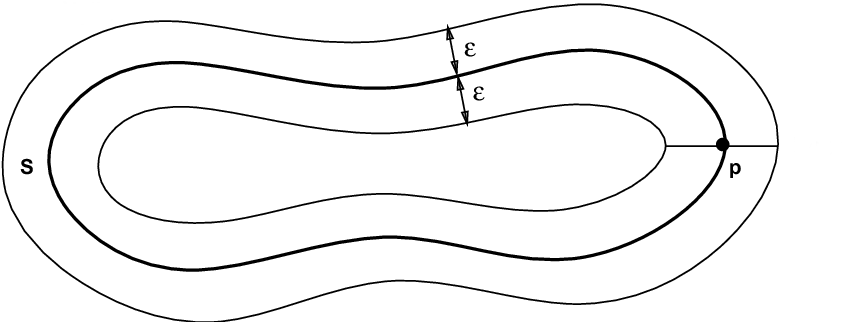
\includegraphics[width=0.9\textwidth]{imagenes/tubular.png}
	\end{center}
	\caption{Entorno tubular}
	\label{fig:etiq_13}
\end{figure}

\begin{teorema}[Existencia de entornos tubulares]
	Sea $S$ una superficie orientable y $R \subset S$ un subconjunto compacto y abierto. Entonces, existe un $\epsilon > 0$ tal que el conjunto $N_{\epsilon}(R) =$ \{todos los segmentos normales centrados en $R$ y longitud $\delta$\}, es un entorno tubular de $R$.
	${ }$\\
	
	En particular, cuando $S$ es compacto, existe un $\epsilon > 0$ tal que $B_{\epsilon}(S)$ es un entorno tubular de $S$.
\end{teorema}




${ }$\\
\subsection{Integración en superficies}
${ }$\\

Ahora recordaremos algunos resultados sobre integración en superficies que serán usados posteriormente.
${}$\\

\begin{teorema}[Fórmula del cambio de variable]
	Sea $F : S_1 \to S_2$ un difeomorfismo, siendo $S_1$, $S_2$ de dos superficies orientables, y sea $\Phi : S_2 \to \mathbb{R}$ una función integrable. Entonces, $(\Phi \circ F)(p)|Jac \Phi|(p)$ es integrable y
	\[
	\int_{S_2} \Phi = \int_{S_1} (\Phi \circ F)|Jac \Phi|.
	\]
\end{teorema}
${ }$\\


Si $S$ es una superficie compacta y conexa y $\Omega$ es el dominio interno determinado por $S$, el teorema de divergencia permite relacionar las integrales de ciertas funciones definidas en $\Omega$ con integrales en la superficie $S$.
${ }$\\

\begin{teorema}[Teorema de la divergencia sobre superficies] \label{teo:divergencia}
	Sea una superficie compacta $S$ y un campo diferenciable de vectores $V : S \to \mathbb{R}^3$. Entonces:
	\begin{enumerate}
		\item $\int_S div V = -2 \int_S \langle V, N \rangle H$,
		\item $\int_S [k_2(p) \langle (dV)_p(e_1), e_1\rangle + k_1(p) \langle (dV)_p(e_2), e_2 \rangle ] \; dp = -2 \int_S \langle V, N \rangle K$, donde $\{ e_1, e_2 \}$
	\end{enumerate}
\end{teorema}
${}$\\

Siendo $div \; V$ la divergencia del campo $V$.
${ }$\\

\begin{teorema}[Fórmulas de Minkowski]
	Sea $S$ una superficie compacta, $N$ su normal interior y $K$, $H$ sus curvaturas de Gauss y media. Entonces, se cumplen las siguientes fórmulas:
	\begin{enumerate}
		\item $\int_S (1 + \langle p, N(p) \rangle H(p) \; dp = 0$,
		\item $\int_S (H(p) + \langle p, N(p) \rangle K(p) \; dp = 0$
	\end{enumerate}
\end{teorema}
${ }$\\







${ }$\\
\subsection{Ovaloides}
${ }$\\

En este epígrafe daremos la definición de ovaloide, así como algunas proposiciones generales de los mismos.
${ }$\\

\begin{definicion}
	Llamaremos \underline{\textbf{ovaloide}} a una superficie $S \subset \mathbb{R}^3$ compacta y conexa cuya curvatura de Gauss sea siempre positiva.
	
	También, si $S$ es un ovaloide, $N =$ normal interior de $S$ y $\sigma =$ segunda forma fundamental respecto a $N$. Entonces, $\sigma > 0$.
\end{definicion}
${ }$\\

\begin{ejemplo} 
	
	Un ejemplo de ovaloide son los elipsoides, veamos que un elipsoide es un ovaloide:
${ }$\\

	Consideremos la función $f : \mathbb{S}^2 \to E$ definida como
	\[
		f(x,y,z) = (ax,by,cz),
	\]
	que nos lleva una esfera en un elipsoide y cuya inversa es $f^{-1} : E \to \mathbb{S}^2$ dada por
	\[
		f^{-1} (x,y,z) = \Big(\frac x a, \frac y b, \frac z c \Big).
	\]
	Esto es posible por que $a,b,c \in \mathbb{R}^3 \setminus \{0\}$ ya que en caso de que alguno de ellos fuese cero tendríamos un elipsoide degenerado.
	${ }$\\
	
	Como podemos observar tanto $f$ como $f^{-1}$ son continuas y por tanto $f$ es un homeomorfismo. Basta recordar que la compacidad y la conexidad son invariantes topológicos y que dichas propiedas se conservan al aplicar homeomorfismos. Así, como la esfera es compacta y conexa el elipsoide también lo es.
	
	
	
		\begin{figure}[h]
			\begin{center}
				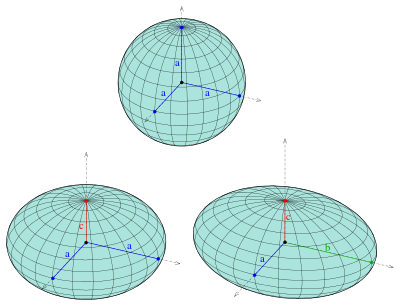
\includegraphics[width=0.8\textwidth]{imagenes/ellipsoid.png}
			\end{center}
			\caption{La elipse es un ejemplo de ovaloide.}
			\label{fig:etiq_3}
		\end{figure}
		
	
	Finalmente, para comprobar que la curvatura de Gauss es siempre positiva usaremos la expresión que se da en el artículo \cite{RonGoldman}:
	$$
		K = - \frac{ \left| {\begin{array}{cc}
				Hess F & \nabla F^t \\ 
				\nabla F & 0 \\
				\end{array} } \right| }{\| \nabla f \|^4}		 
	$$
	En nuestro caso, tenemos
	\[
		K = - \frac{ \left| {\begin{array}{cccc}
				2/a^2 & 0 & 0 & 2x/a^2 \\ 
				0 & 2/b^2 & 0 & 2y/b^2 \\ 
				0 & 0 & 2/c^2 & 2z/c^2 \\ 
				2x/a^2 & 2y/b^2 & 2z/c^2 & 0 \\
				\end{array} } \right| }{\| \nabla f \|^4}
		= \frac{16}{a^4b^4c^4 \| \nabla f \|^4}(a^2 b^2 z^2+a^2c^2y^2+b^2c^2x^2),
	\]
	que es siempre positivo.
\end{ejemplo}
${ }$\\

\begin{ejemplo}
	Otro ejemplo de ovaloide es el dado por la ecuación $$ x^4 + y^4 + z^4 = 1 $$ la gráfica de esta ecuación está representada en la Figura \ref{fig:etiq_11}.
		\begin{figure}[ht]
			\begin{center}
				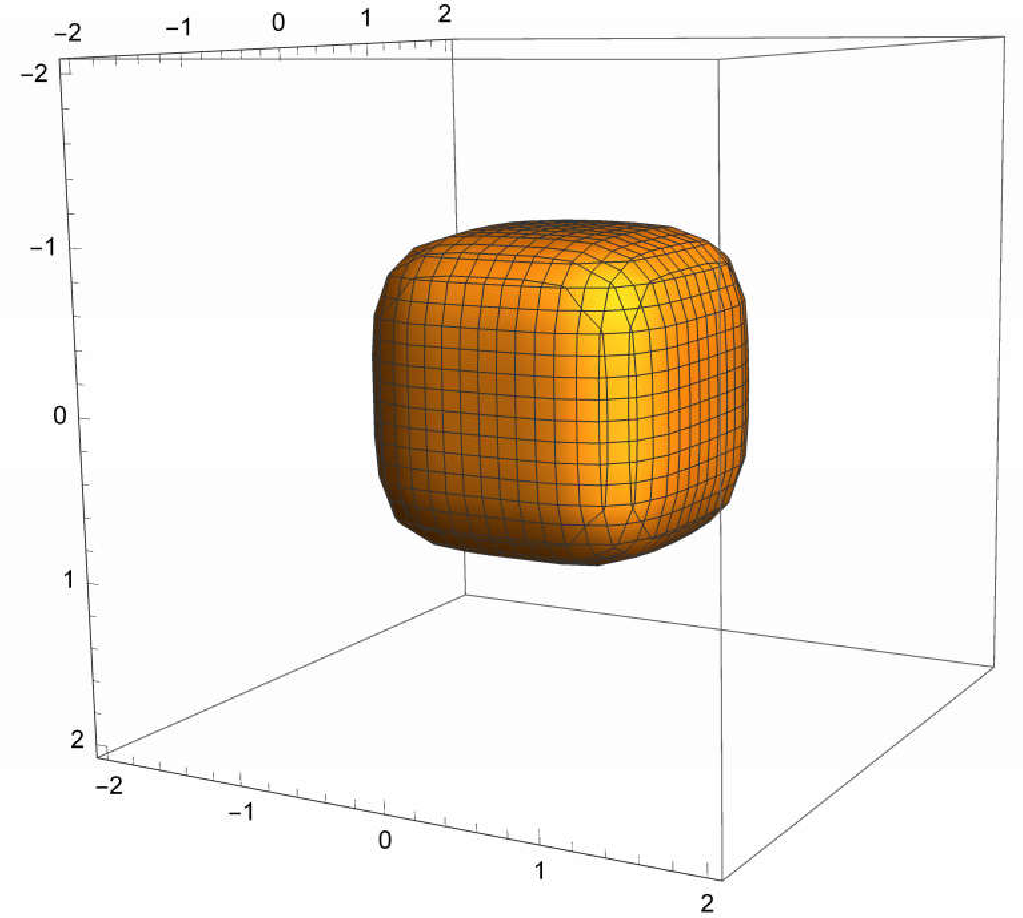
\includegraphics[width=0.8\textwidth]{imagenes/ovaloide2.png}
			\end{center}
			\caption{Ovaloide de ecuación $x^4 + y^4 + z^4 = 1$ en Mathematica.}
			\label{fig:etiq_11}
		\end{figure}
\end{ejemplo}
${ }$\\

Para hacernos una idea mas concreta de que forma tendrá un ovaloide podemos observar que este es homeomorfo a la esfera según aparece en la bibliografía \cite{ref1}. Recordemos también que homeomorfo implica homotópico.
${ }$\\

El siguiente resultado afirma que el dominio interno de una superficie conexa y cerrada con curvatura de Gauss positiva es convexo.
${ }$\\

\begin{teorema}[Hadamard-Stoker] \label{teo:hadamard}
	Sea un ovaloide $S \subset \mathbb{R}^3$ y $\Omega$ su dominio interior. Entonces:
	
	\begin{enumerate}
		\item Para todo $x, y \in \overline{\Omega}$. Entonces, el segmento que los une $]x, y[ \subset \Omega$. En particular, $\Omega$ es convexo.
		\item Para cada $p \in S$, $\Pi_p \cap S = \{p\}$, donde $\Pi_p$ es el plano tangente afín a $S$ en p. Además, $\overline{\Omega} \subset \bigcap_{p \in S} \; \Pi^{+}_{p}$.
	\end{enumerate}
\end{teorema}
${ }$\\

\begin{teorema}[Hadamard]
	Sea $S$ un ovaloide, entonces la aplicación de Gauss $N : S \to \mathbb{S}^2$ es un difeomorfismo. En particular, $S$ es difeomorfa a una esfera.
\end{teorema}
${ }$\\


${ }$\\
\subsection{Superficie rígida}
%$\textbf{1.1.2. Superficie rígida}$
${ }$\\

\begin{definicion}
	Diremos que $S \subset \mathbb{R}^3$ es una \underline{\textbf{superficie rígida}} cuando toda isometría $f : S \to S'$ sea la restricción de un movimiento rígido, esto es, existe un movimiento rígido $F : \mathbb{R}^3 \to \mathbb{R}^3$ tal que $f = F_{|S}$.
\end{definicion}
${ }$\\

Dicho esto, las superficies rígidas son aquellas que, al aplicarles una isometría $f : S \to S'$, conservan la distancia entre puntos y también las curvaturas de las secciones normales de la superficie luego la superficie no puede ser ni estirada (no conservaría distancias) ni deformada (no conservaría curvaturas para cada uno de sus puntos) dejando solo la posibilidad de ser girada y trasladada en el espacio esto nos permitirá extender esta función a un movimiento rígido de $\mathbb{R}^3$.
${ }$\\



%%% VOLVER A MIRAR ESTE PARRAFO PARA CORREGIRLO
En el ejemplo de superficie no rígida de la Figura\ref{fig:etiq_2}, podemos ver que hay un plano por el cual el trozo de superficie que se encuentra a uno de los lados puede ser cambiada por su simétrico con respecto a este plano creando una nueva superficie deformada de la anterior, pero que conserva la distancia de los puntos en el sentido que se dijo de la isometría. Está función que ha sido aplicada a la superficie es por tanto una isometría, pero no es un movimiento rígido ya que en los puntos que han sido modificados por esta simetría la superficie a cambiado su curvatura.
${ }$\\

%Como acabamos de ver la rigidez es una propiedad de las esferas, aunque no es exclusiva para las esferas sino para mas superficies entre ellas los ovaloides (como veremos mas adelante). Sin embargo, hay superficies que no tienen esta propiedad de rigidez como se puede observar en el ejemplo que se muestra en la Figura \ref{fig:etiq_2}

\begin{figure}[h]
	\begin{center}
		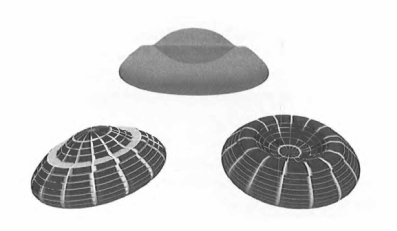
\includegraphics[width=0.8\textwidth]{imagenes/no_rigid}
	\end{center}
	\caption{Superficie no rígida.}
	\label{fig:etiq_2}
\end{figure}



${ }$\\
${ }$\\
${ }$\\
\section{Visualización de superficies}
${ }$\\

Las ecuaciones paramétricas que definen una superficie podrían ser vistas como una función a la que, pasándole una tupla te devuelven uno de los puntos que está en la superficie. Veamos la siguiente representación:
${ }$\\
$$ x = x(u,v) $$
$$ y = y(u,v) $$
$$ z = z(u,v). $$
${ }$\\
Del mismo modo que con las ecuaciones paramétricas que definen superficies, podríamos ver las ecuaciones implícitas que definen una superficie, como una función que a partir de un punto del espacio indica si dicho punto esta fuera o dentro de la superficie.
${ }$\\

Poniendo como ejemplo a la esfera, que puede definirse de cualquiera de las siguientes dos formas
${ }$\\
$$ {x_1}^2 + {x_2}^2 + {x_3}^2 -1 = 0, $$
$$ \lVert \mathbf{x} \rVert -1 = 0, $$
${ }$\\
donde $x = (x_1, x_2, x_3)$. La segunda definición en forma implícita de la esfera concuerda con la primera en todos los puntos que pertenecen a la esfera, pero difiere en los demás. La primera de ellas define la distancia algebraica mientras que la otra define la distancia geométrica o euclidea.
${ }$\\

¿Cual de las representaciones anterior podría ser mejor que la otra? En el artículo \ref{JHart} se puede leer lo siguiente:
${ }$\\

``A comparison of geometric versus algebraic representations of quadric surfaces preferred the geometric representation [Goldman, 1983]. The parameters of a geometric representation are coordinate-independent, and are more robust and intuitive than algebraic coefficients. Distance-based functions like (2) are one method for representing implicit surfaces geometrically.

Several methods exist for rendering implicit surfaces. Indirect methods polygonize the implicit surface to a given tolerance, allowing the use of existing polygon rendering techniques and hardware for interactive inspection [Wyvill et al, 1986; Bloomenthal, 1988]. Although polygonization transforms implicit surfaces into a representation easily rendered and incorporated into graphics systems, polygonizations are typically not guaranteed and may not accurately detect disconnected or detailed sections of the implicit surface. Production ray tracing systems tend to polygonize surfaces, resulting in large time and memory overhead to accurately represent an otherwise simple implicit model.

In an effort to combine speed and accuracy, [Sederberg \& Zundel, 1989] developed a direct scan-line method to more accurately render algebraic implicit surfaces at interactive speeds. Ray tracing, on the other hand, is a direct, accurate and elegant method for investigating a much larger variety of implicit surfaces.''
${ }$\\

A lo largo de este capítulo veremos como rayos, $ r : \mathbb{R} \to \mathbb{R}^3$, definidos como
${ }$\\
$$ r(t) = o + dt $$
${ }$\\
intersectan superficies definidas con ecuaciones implícitas. Si tenemos una superficie dada por $ F : \mathbb{R}^3 \to \mathbb{R} $
${ }$\\
$$ F(x,y,z) = 0, $$
${ }$\\
obtenemos la intersección con el rayo usando la composición $F \circ r : \mathbb{R} \to \mathbb{R}$, $F \circ r (t) = 0$, cuyas raíces corresponden con las intersecciones del rayo con la superficie.
${ }$\\

Hay superficies sencillas como la esfera y el cubo cuya intersección es fácil de calcular directamente, pero hay casos de funciones en los que no se puede calcular directamente despejando variables, en estos caso recurrimos a métodos de aproximación de soluciones como son el método de Newton-Raphson y el método de Regula-Falsi.
${ }$\\

Estos métodos parten de una aproximación inicial de la solución y generan una sucesión de términos que converge a la solución.